% This file was created with tikzplotlib v0.10.1.
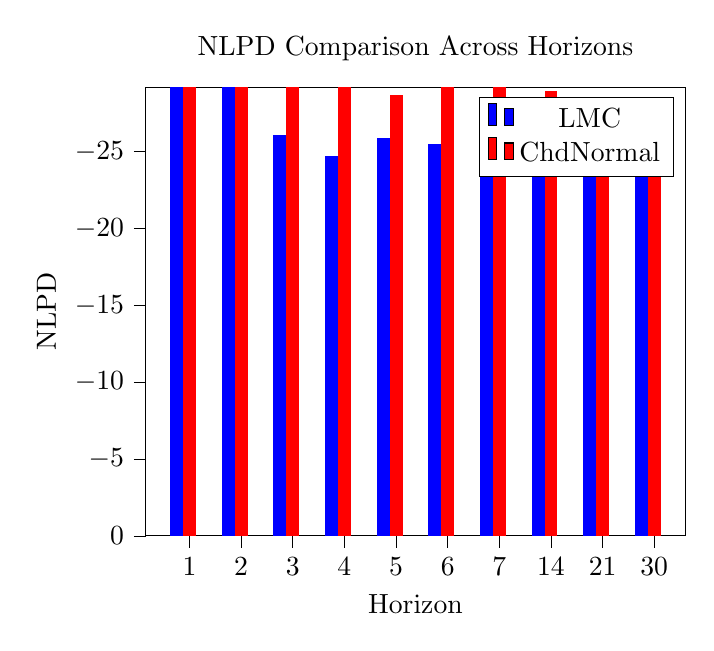
\begin{tikzpicture}

\definecolor{darkgray176}{RGB}{176,176,176}

\begin{axis}[
tick align=outside,
tick pos=left,
title={NLPD Comparison Across Horizons},
x grid style={darkgray176},
xlabel={Horizon},
xmin=-0.85, xmax=9.6,
xtick style={color=black},
xtick={0,1,2,3,4,5,6,7,8,9},
xticklabels={1,2,3,4,5,6,7,14,21,30},
y dir=reverse,
y grid style={darkgray176},
ylabel={NLPD},
ymin=-29.1668841658586, ymax=0,
ytick style={color=black}
]
\draw[draw=none,fill=blue] (axis cs:-0.375,0) rectangle (axis cs:-0.125,-32.745747598516);
\addlegendimage{ybar,ybar legend,draw=none,fill=blue}
\addlegendentry{LMC}

\draw[draw=none,fill=blue] (axis cs:0.625,0) rectangle (axis cs:0.875,-30.2613167702501);
\draw[draw=none,fill=blue] (axis cs:1.625,0) rectangle (axis cs:1.875,-26.0674625485646);
\draw[draw=none,fill=blue] (axis cs:2.625,0) rectangle (axis cs:2.875,-24.7284934760365);
\draw[draw=none,fill=blue] (axis cs:3.625,0) rectangle (axis cs:3.875,-25.8667874240686);
\draw[draw=none,fill=blue] (axis cs:4.625,0) rectangle (axis cs:4.875,-25.5241222520839);
\draw[draw=none,fill=blue] (axis cs:5.625,0) rectangle (axis cs:5.875,-24.4733528784515);
\draw[draw=none,fill=blue] (axis cs:6.625,0) rectangle (axis cs:6.875,-23.7189187161835);
\draw[draw=none,fill=blue] (axis cs:7.625,0) rectangle (axis cs:7.875,-24.6262096068829);
\draw[draw=none,fill=blue] (axis cs:8.625,0) rectangle (axis cs:8.875,-24.551868432483);
\draw[draw=none,fill=red] (axis cs:-0.125,0) rectangle (axis cs:0.125,-37.1976418206135);
\addlegendimage{ybar,ybar legend,draw=none,fill=red}
\addlegendentry{ChdNormal}

\draw[draw=none,fill=red] (axis cs:0.875,0) rectangle (axis cs:1.125,-32.57009392034);
\draw[draw=none,fill=red] (axis cs:1.875,0) rectangle (axis cs:2.125,-31.1545299186111);
\draw[draw=none,fill=red] (axis cs:2.875,0) rectangle (axis cs:3.125,-30.7281603098309);
\draw[draw=none,fill=red] (axis cs:3.875,0) rectangle (axis cs:4.125,-28.7134159542646);
\draw[draw=none,fill=red] (axis cs:4.875,0) rectangle (axis cs:5.125,-29.5248659053096);
\draw[draw=none,fill=red] (axis cs:5.875,0) rectangle (axis cs:6.125,-29.6611175531187);
\draw[draw=none,fill=red] (axis cs:6.875,0) rectangle (axis cs:7.125,-28.9486441224176);
\draw[draw=none,fill=red] (axis cs:7.875,0) rectangle (axis cs:8.125,-27.8247484458317);
\draw[draw=none,fill=red] (axis cs:8.875,0) rectangle (axis cs:9.125,-26.5153492416896);
\end{axis}

\end{tikzpicture}
